\chapter{Praktični rad}

U iBeacon poglavlju spomenuto je kako se tehnologija iBeacon može iskoristiti u gotovo svim situacijama gdje se sadržaj mijenja ovisno o kontekstu prostora, npr. trgovinama, muzejima, bolnicama i sličnim objektima. 
\\
U nastavku poglavlja opisano je kako se tehnologija iBeacon može integrirati u trgovine. 
\\

Za integraciju je potrebno imati postavljene iBeacon uređaje u prostoru, klijentsku mobilnu aplikaciju koja može prepoznati BLE, odnosno iBeacon, odašiljače te poslužiteljsku aplikaciju s koje će mobilni uređaj dohvaćati relevantne podatke.  

\section*{Poslužiteljska aplikacija}

Spree Commerce (u daljnjem tekstu Spree) je elektronička trgovina \engl{e-commerce} otvorenog koda napisana u Ruby on Rails radnom okruženju. 
Rad na Spreeu je počeo 2007. godine, a danas je jedna od najpopularnijih platformi za elektroničku trgovinu. 
Trenutno više od 45 tisuća trgovina koristi Spree. %TODO reff http://spreecommerce.com/storefront 
\\
Odlike Spree rješenja su ogroman broj već implementiranih funkcija koje imaju sve moderne elektroničke trgovine, modularan programski kôd, lakoća dodavanja novih funkcionalnosti te izmjena i konfiguracija postojećih te brojne druge. 
Uz to, za gotovo svaki aspekt sustava dostupan je skup aplikacijsko programskih sučelja što pojednostavljuje integraciju sustava sa drugim tehnologijama (poput integracije sa mobilnim platformama).
\\

\begin{figure}[H]
    \centering
    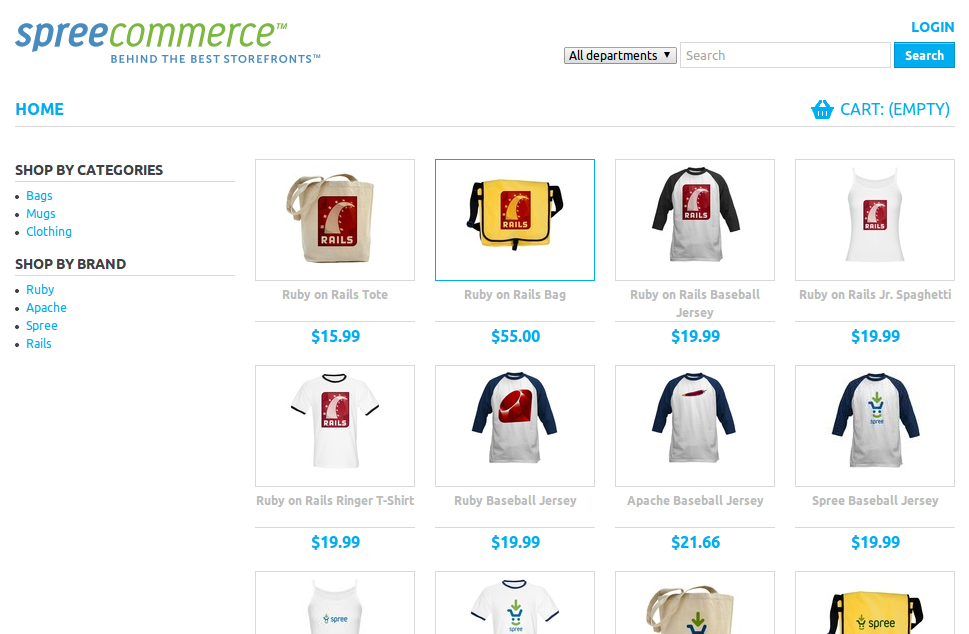
\includegraphics[scale=0.40]{pictures/spree}
    \caption{Početni ekran Spree korisničkog sučelja}
    \label{pic:spree}
\end{figure}

\begin{figure}[H]
    \centering
    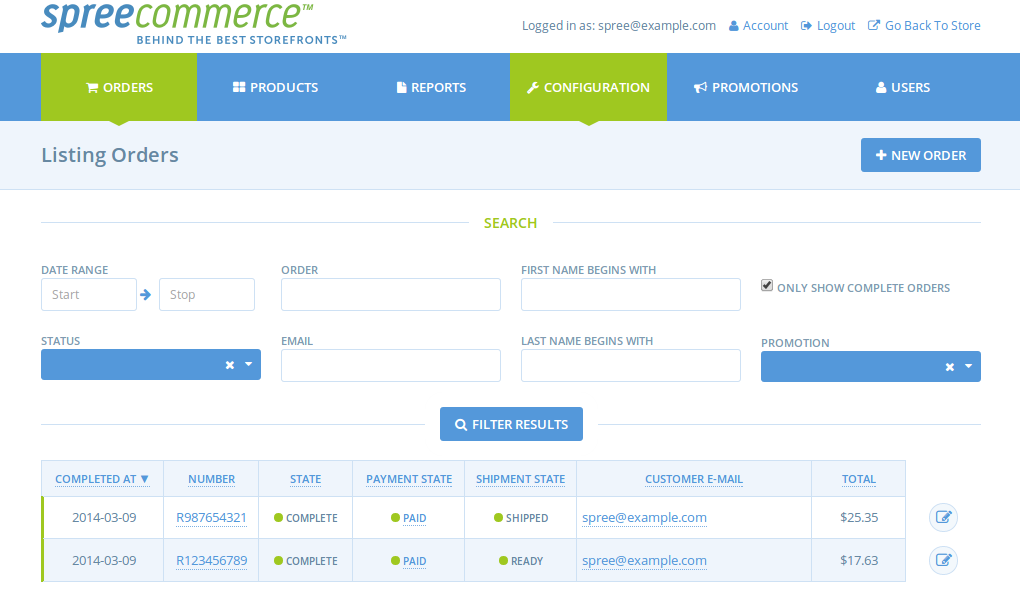
\includegraphics[scale=0.40]{pictures/spree_admin}
    \caption{Početni ekran Spree administratorskog sučelja}
    \label{pic:spree}
\end{figure}

\begin{figure}[H]
    \centering
    
\includegraphics[scale=0.65]{pictures/spree_lavazza}
    \caption{Lavazza Store - jedna od mnogobrojnih elektroničkih trgovina koje koriste Spree}
    \label{pic:spreeLavazza}
\end{figure}

Spree je podijeljen na nekoliko ključnih komponenti (tj. Ruby Gemova):
\begin{description}[style=nextline]
    \item[spree\_api] Skup aplikacijsko programskih sučelja koji zadovoljavaju REST\footnote{\textit{Representational State Transfer}, \url{http://en.wikipedia.org/wiki/Representational_state_transfer}} principe.
    \item[spree\_frontend] Komponente korisničkog sučelja.
    \item[spree\_backend] Komponente korisničkog sučelja administratora aplikacije.
    \item[spree\_cmd] Komponente sučelja naredbenog retka \engl{command-line interface, CLI}.
    \item[spree\_core] Ključne komponente, sadrži veliku većinu poslovne logike.
    \item[spree\_sample] Primjeri podataka.
\end{description}

Ako programer želi dodati neku od Spree komponenti u svoju postojeću aplikaciju, sve što treba napraviti je dodati željene komponente u Gemfile\footnote{datoteka koja sadrži popis svih Ruby Gemova koji se koriste u projektu} te pokrenuti instalaciju.

%TODO instalacija railsa i spreea 


%TODO dijelovi spreea
%TODO spree_taxon_web_services
%TODO instalacija aplikacije
%TODO pokretanje aplikacije

\section*{Klijentska aplikacija}

%TODO uvod
%TODO integriranje aplikacije sa ibeaconima, use caseovi
%TODO spajanje aplikacije sa serverom
%TODO instalacija i pokretanje aplikacije
%TODO eksperimentalna aplikacija